\documentclass[letterpaper]{article} % DO NOT CHANGE THIS
\usepackage[submission]{aaai2027}  % DO NOT CHANGE THIS
\usepackage[hyphens]{url}  % DO NOT CHANGE THIS
\usepackage{graphicx} % DO NOT CHANGE THIS
\urlstyle{rm} % DO NOT CHANGE THIS
\def\UrlFont{\rm}  % DO NOT CHANGE THIS
\usepackage{natbib}  % DO NOT CHANGE THIS AND DO NOT ADD ANY OPTIONS TO IT
\usepackage{caption} % DO NOT CHANGE THIS AND DO NOT ADD ANY OPTIONS TO IT
\frenchspacing  % DO NOT CHANGE THIS
\usepackage{amsmath}
\usepackage{amssymb}
\usepackage{amsthm}
\usepackage{booktabs}
\usepackage{array}
\usepackage[table]{xcolor}

\definecolor{pennblue}{HTML}{011F5B}
\definecolor{pennred}{HTML}{990000}
\definecolor{controlgray}{HTML}{7F7F7F}
\newcommand{\helpful}[1]{\textcolor{pennblue}{\bfseries #1}}
\newcommand{\utilityhelpful}[1]{\textcolor{pennblue}{\bfseries #1}}
\newcommand{\harmful}[1]{\textcolor{pennred}{\bfseries #1}}
\newcommand{\neutral}[1]{\textcolor{controlgray}{#1}}
\newcommand{\diagnostic}[1]{\textcolor{controlgray}{#1}}

\newtheorem{theorem}{Theorem}
\newtheorem{corollary}[theorem]{Corollary}

\renewcommand{\thesection}{S\arabic{section}}
\renewcommand{\thesubsection}{S\arabic{section}.\arabic{subsection}}
\renewcommand{\thefigure}{S\arabic{figure}}
\renewcommand{\thetable}{S\arabic{table}}
\renewcommand{\thetheorem}{S\arabic{theorem}}

\pdfinfo{
/TemplateVersion (2027.1)
}

\title{Supplementary Material: Fixed-Spectrum Attention Routing for Length-Generalizing Retrieval}
\author{Anonymous Submission}
\affiliations{}
\nocopyright

\begin{document}
\maketitle

This document supplies proofs, experimental protocols, complete result tables, secondary figures, negative
replications, and reproducibility information for the main paper. The main paper is self-contained; this
supplement preserves the full audit trail behind its compressed claims.

\section{Theory Details}

\subsection{Established softmax grouping identity}

For evidence positions $S$, distractors $D$, scores $s_j$, and temperature $T>0$, let
$Z_G=\sum_{j\in G}e^{s_j/T}$ and $F_G=-T\log Z_G$. Direct grouping of the softmax denominator gives
\begin{equation}
m_S:=\sum_{j\in S}a_j
=\frac{Z_S}{Z_S+Z_D}
=\sigma\!\left(\frac{F_D-F_S}{T}\right).
\label{eq:supp-free-energy}
\end{equation}
Defining the group log-mean-exp score
$\bar s_G=T\log(|G|^{-1}\sum_{j\in G}e^{s_j/T})$ yields the exact threshold relation
\begin{equation}
m_S\ge\alpha
\Longleftrightarrow
\bar s_S-\bar s_D\ge
T\left(\log\frac{|D|}{|S|}+\operatorname{logit}(\alpha)\right).
\label{eq:supp-length-cost}
\end{equation}
These are standard Gibbs or partition-function identities \citep{ramsauer2021hopfield}. They motivate the
competition for evidence mass and position the paper. Equation~\ref{eq:supp-length-cost} also prevents
an overstatement: distractor count alone is insufficient because arbitrarily many negligible-score
distractors need not reduce evidence mass.

\subsection{Fixed-spectrum routing range}

Let $a_{(1)}\ge\cdots\ge a_{(n)}$, let $S$ contain $r$ evidence positions, and define
\begin{equation}
\begin{aligned}
C_r^+&=\sum_{i=1}^ra_{(i)},\qquad
C_r^-=\sum_{i=n-r+1}^na_{(i)},\\
K_r&=C_r^+-C_r^-.
\end{aligned}
\end{equation}

\begin{theorem}[Capacity--assignment decomposition]
For every permutation $\pi$ of a fixed attention-weight multiset,
$C_r^-\le m_S(\pi)\le C_r^+$, both endpoints are attainable, and for $K_r>0$ the unique coordinate
\begin{equation}
\rho_S(\pi)=\frac{m_S(\pi)-C_r^-}{K_r}\in[0,1]
\end{equation}
gives $m_S(\pi)=C_r^-+\rho_S(\pi)K_r$.

For affine margin $M(\pi)=b+\sum_ja_{\pi(j)}u_j$, sorted utilities
$u_{(1)}\ge\cdots\ge u_{(n)}$ give
\begin{align}
\max_\pi M(\pi)&=b+\sum_i a_{(i)}u_{(i)},\\
\min_\pi M(\pi)&=b+\sum_i a_{(i)}u_{(n+1-i)}.
\end{align}
No statistic invariant to token permutation can determine evidence assignment or the output margin.
\end{theorem}

\begin{proof}
An $r$-position set receives at most the $r$ largest weights and at least the $r$ smallest; assigning those
weights to $S$ attains the endpoints. Normalizing the bounded mass gives $\rho_S$. For the output range,
suppose $u_p>u_q$ but $a_{\pi(p)}<a_{\pi(q)}$. Swapping those weights changes the margin by
$(a_{\pi(q)}-a_{\pi(p)})(u_p-u_q)>0$. Repeated exchanges align weights and utilities for the maximum and
reverse them for the minimum, the classical rearrangement inequality \citep{hardylittlewoodpolya1952}.
The extremal assignments preserve the complete weight multiset and therefore every permutation-invariant
statistic.
\end{proof}

\subsection{Nonlinear downstream network}

Fix an input and selected heads $H$ at one layer. Let $x_{hj}=O_hv_{hj}$ and
$z=\sum_{h\in H}\sum_j a_{hj}x_{hj}$. For target $y$ and competitor $c$, let
$M_c(z)=g_y(z)-g_c(z)$. A source--donor swap has
\begin{equation}
\delta_h=a_{hd_h}-a_{hs},\qquad
\Delta z=\sum_{h\in H}\delta_h(x_{hs}-x_{hd_h}).
\end{equation}
Define local utility $u_{hj}^{(c)}=\nabla M_c(z)^\top x_{hj}$.

\begin{theorem}[Nonlinear routing-margin bound]
If $\nabla M_c$ is $L_c$-Lipschitz from $z$ to $z+\Delta z$, then
\begin{equation}
\left|\Delta M_c-
\sum_{h\in H}\delta_h(u_{hs}^{(c)}-u_{hd_h}^{(c)})\right|
\le\frac{L_c}{2}\lVert\Delta z\rVert_2^2.
\label{eq:supp-nonlinear}
\end{equation}
\end{theorem}

\begin{proof}
The swap changes head $h$ by exactly $\delta_h(x_{hs}-x_{hd_h})$. The fundamental theorem of calculus gives
\begin{equation}
\Delta M_c=\int_0^1\nabla M_c(z+t\Delta z)^\top\Delta z\,dt.
\end{equation}
Subtracting $\nabla M_c(z)^\top\Delta z$ and applying Lipschitzness bounds the remainder by
$\int_0^1L_ct\lVert\Delta z\rVert_2^2dt=L_c\lVert\Delta z\rVert_2^2/2$
\citep{nesterov2004}. Expanding the first-order term gives Equation~\ref{eq:supp-nonlinear}.
\end{proof}

\begin{corollary}[Multi-evidence routing]
Let $S$ contain $r$ evidence positions and pair every evidence position missing a top-$r$ weight with one
top-$r$ non-evidence donor. For disjoint swap pairs $P_h$ and
$\delta_{hsd}=a_{hd}-a_{hs}\ge0$,
\begin{equation}
\Delta z=\sum_{h\in H}\sum_{(s,d)\in P_h}\delta_{hsd}(x_{hs}-x_{hd}),
\end{equation}
and Equation~\ref{eq:supp-nonlinear} holds with the first-order sum extended over $(s,d)\in P_h$.
Thus assigning top-$r$ capacity to the evidence improves the margin whenever the summed evidence--donor
utility gain exceeds the curvature remainder.
\end{corollary}

The condition is sufficient, not necessary. Source-max can fail when evidence values have no greater
downstream utility, patched heads cancel, or curvature dominates. This is why natural source mass is not a
universal circuit-selection rule.

\section{Controlled Experiments}

\subsection{Tasks and training}

\textbf{Argmax retrieval} presents key--value pairs and requests the value paired with the largest key.
\textbf{Flag retrieval} presents values with exactly one marked position and requests the marked value.
Both tasks are order-invariant and have one identifiable evidence position. \textbf{Reversed decimal
addition} is an order-dependent contrast. \textbf{Two-evidence modular sum} marks two digits and requests
their sum modulo ten, so copying either digit is insufficient.

The primary model is a four-layer pre-norm decoder transformer with width $256$, eight heads, and feed-forward
width $1024$. We train with AdamW, batch size $512$, and warmup plus cosine decay on lengths one through five.
Evaluation follows a geometric ladder to $50\times$ training length. The scale replication uses eight layers
and width $512$. A cell is interpreted only after training-length exact match reaches $0.8$. Order-invariant
cells use four seeds; the order-dependent contrast uses two. The preregistration fixes the competence gate,
break-point rule, and variance-collapse check before intervention outcomes.

\subsection{Measured quantities and interventions}

At the answer query we record evidence mass, attention entropy, every attention norm, participation ratio,
attention-output variance, and target margins. The variance intervention replaces
$h\leftarrow h+z$ with $h\leftarrow h+\mathrm{LN}(z)$ after attention, holding the downstream variance of
$z$ approximately constant. The concentration intervention applies length-scaled logit sharpening.

For the fixed-spectrum test, source-max swaps the source weight with the row maximum, source-min swaps it
with the row minimum, and the distractor control swaps the largest and smallest non-source weights. All
conditions preserve model parameters, prompts, transformed values, the complete sorted attention row,
entropy, norms, maximum, and participation ratio. The control additionally preserves source mass.

\subsection{Observational and variance-control results}

Attention on the correct source predicts per-token accuracy with pooled correlation $0.94$ and mean
within-cell correlation $0.97$. Attention-output variance also collapses, but reaches $0.45$ pooled and
$0.59$ within cell. The variance intervention holds the post-intervention ratio near one while behavior remains
accuracy (Table~\ref{tab:supp-variance}).

\begin{figure}[t]
\centering

\includegraphics[width=0.96\columnwidth]{figures/fig_causal.png}
\caption{Controlled baselines pooled over lengths and seeds. Accuracy is tightly related to attention on the
task-required source (top), but only diffusely related to attention-output variance (bottom).}
\label{fig:supp-localization}
\end{figure}

\begin{table*}[t]
\centering
\small
\begin{tabular}{llcccccc}
\toprule
Task & PE, intervention & $1\times$ & $3\times$ & $10\times$ & $50\times$ & Var. (pre, post) & Effect at $50\times$ \\
\midrule
Argmax & NoPE, off & 1.00 & .98 & .83 & .59 & $.33,.33$ & n/a \\
       & NoPE, on  & 1.00 & .97 & .80 & .58 & $.20,.99$ & $-.013$ \\
       & RoPE, off & 1.00 & .95 & .77 & .60 & $.27,.27$ & n/a \\
       & RoPE, on  & 1.00 & .96 & .67 & .57 & $.45,1.00$ & $-.033$ \\
\midrule
Flag   & NoPE, off & 1.00 & .94 & .67 & .60 & $.47,.47$ & n/a \\
       & NoPE, on  & 1.00 & .88 & .62 & .52 & $.49,1.00$ & $-.081$ \\
       & RoPE, off & 1.00 & .99 & .65 & .56 & $.48,.48$ & n/a \\
       & RoPE, on  & 1.00 & .96 & .53 & .50 & $.43,1.00$ & $-.061$ \\
\bottomrule
\end{tabular}
\caption{Controlled retrieval accuracy and variance stabilization. The variance columns report the long-
length ratio before and after normalization. Behavior remains impaired after the statistic is repaired.}
\label{tab:supp-variance}
\end{table*}

\begin{figure*}[t]
\centering
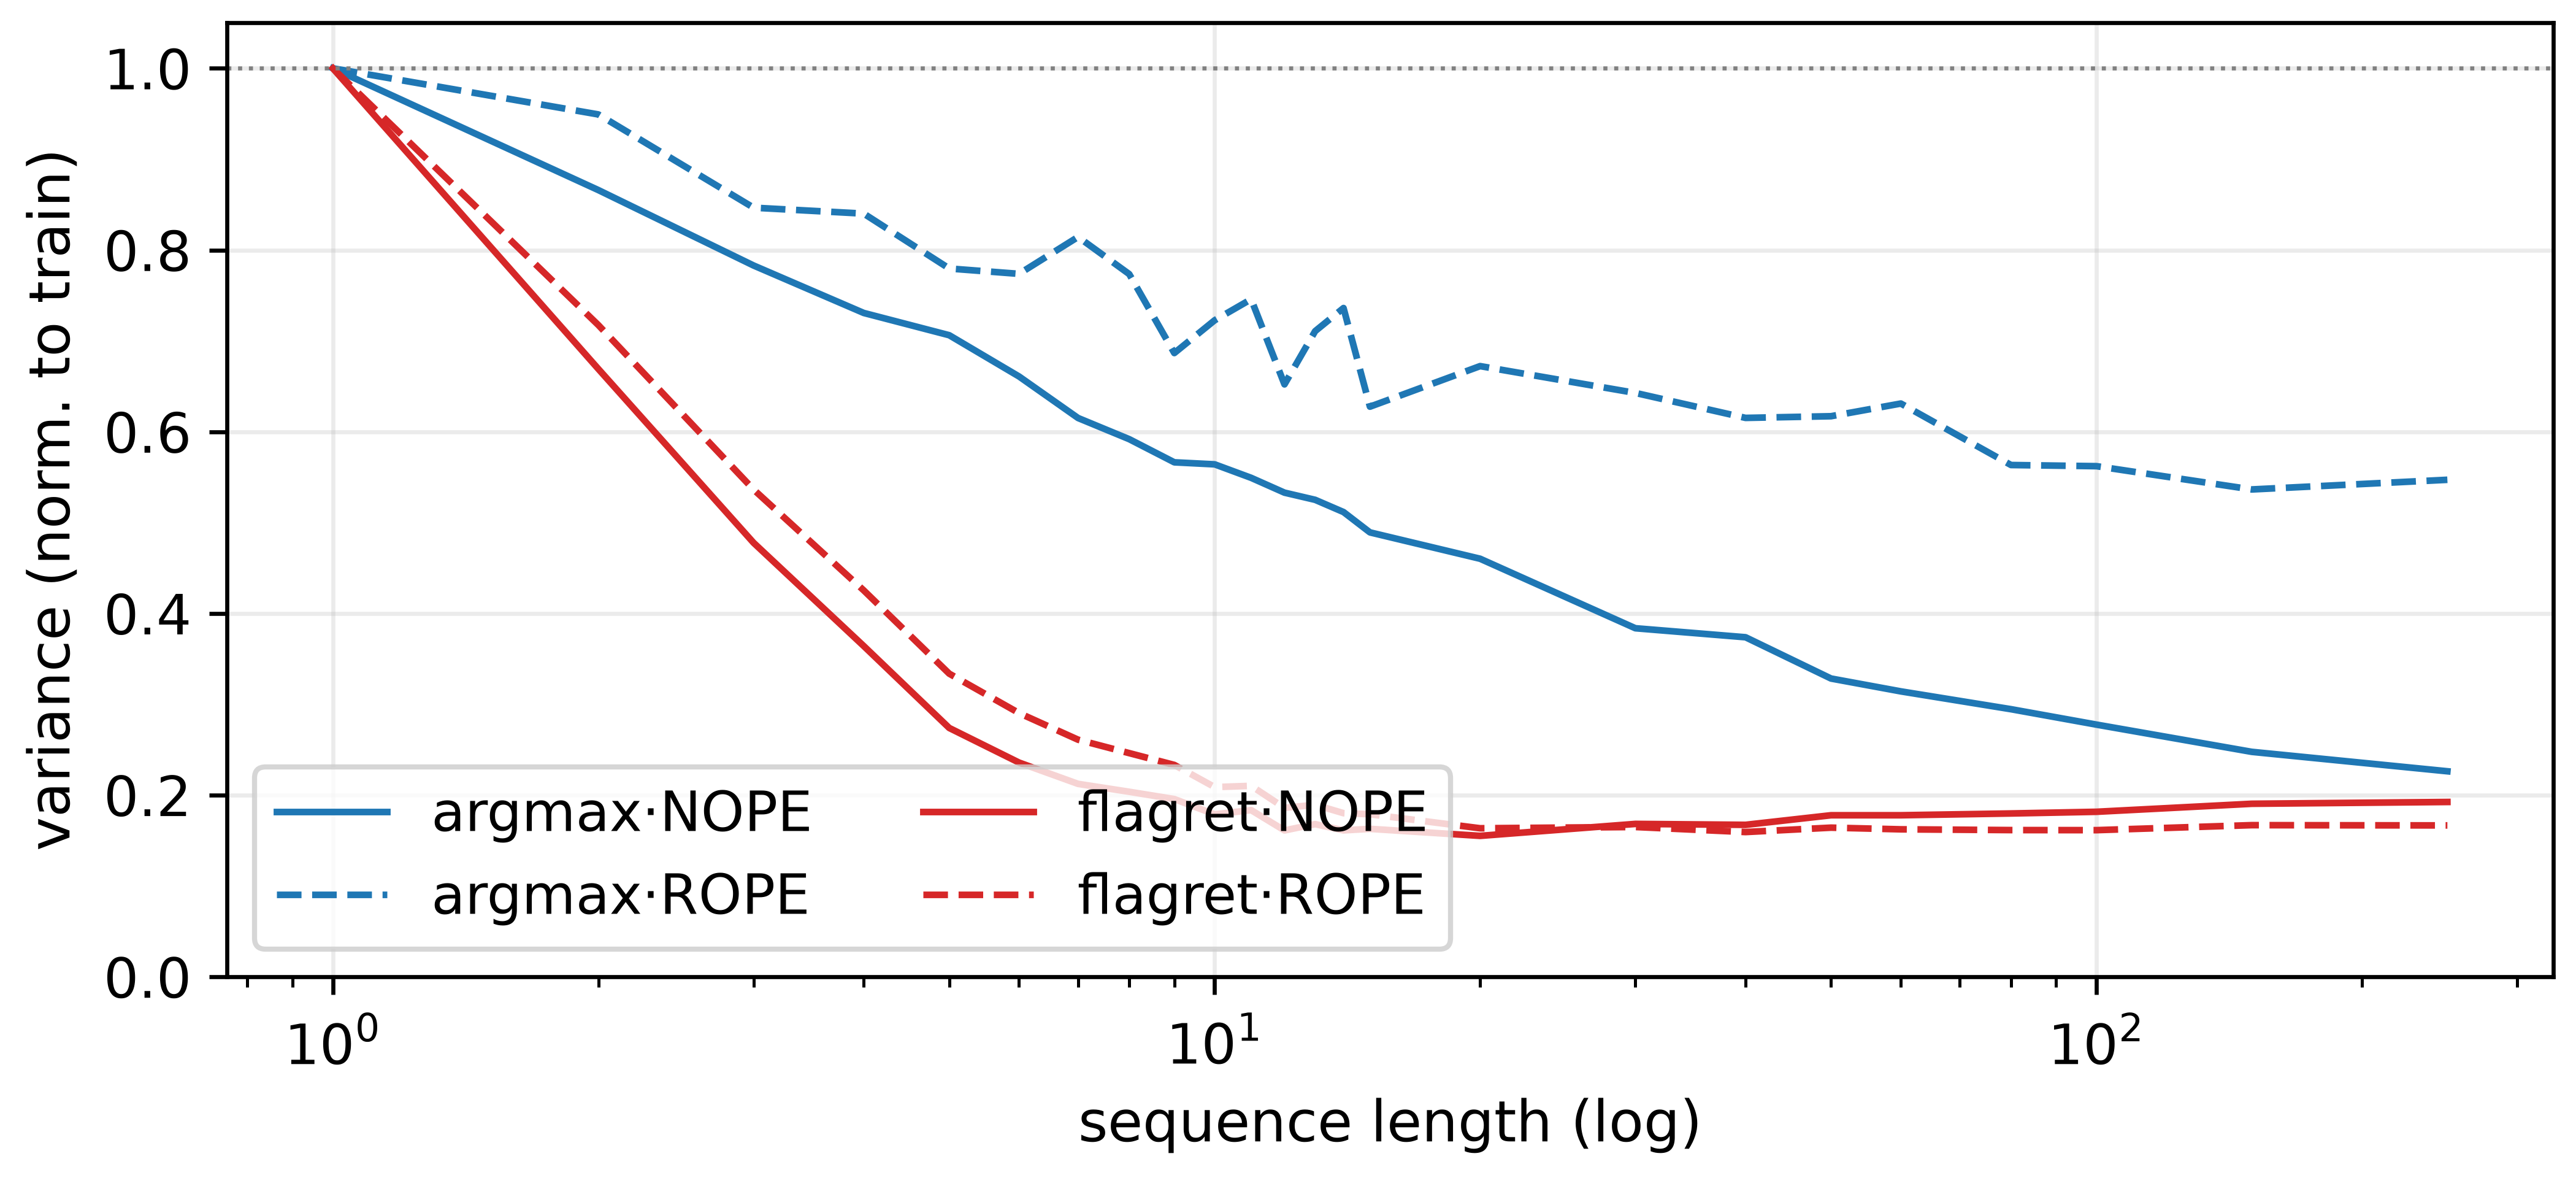
\includegraphics[width=0.82\textwidth]{figures/fig_variance_collapse.png}
\caption{Baseline attention-output variance collapses with length on every controlled task.}
\label{fig:supp-var}
\end{figure*}

\begin{figure*}[t]
\centering
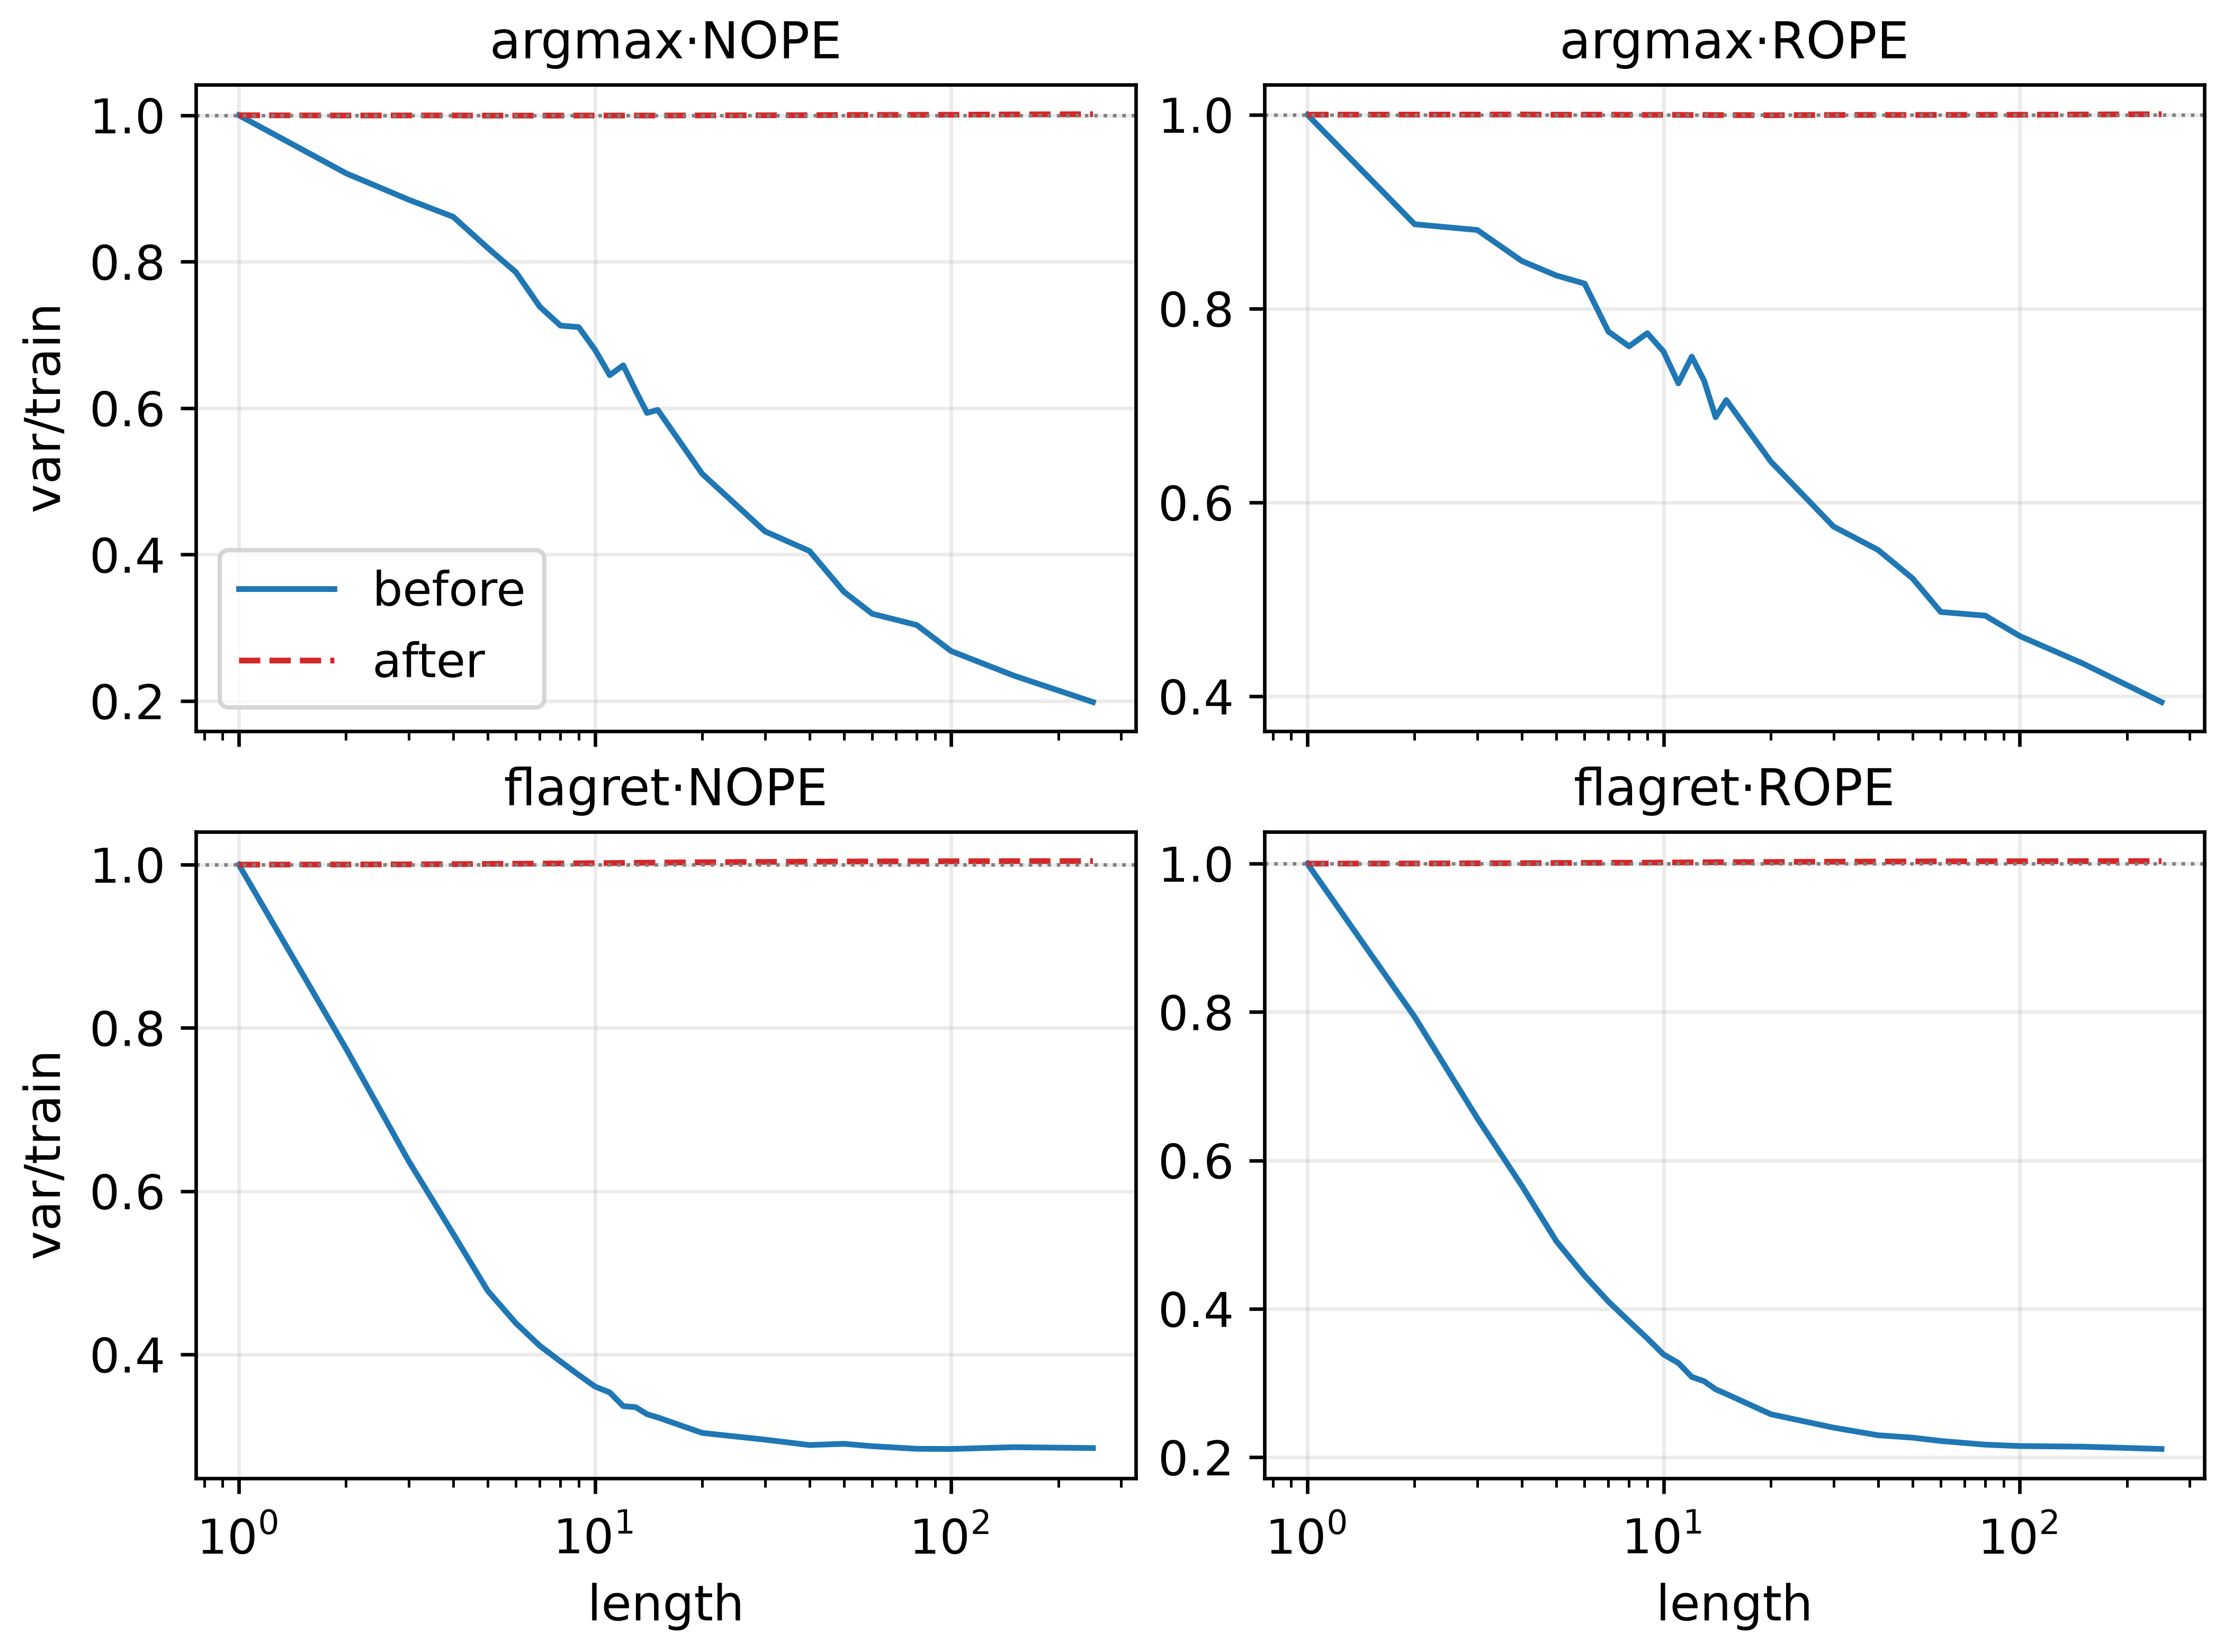
\includegraphics[width=0.82\textwidth]{figures/fig_prepost_var.png}
\caption{The variance intervention works mechanically: raw variance still collapses while normalized
variance remains near its training-length scale.}
\label{fig:supp-prepost}
\end{figure*}

\begin{figure*}[t]
\centering
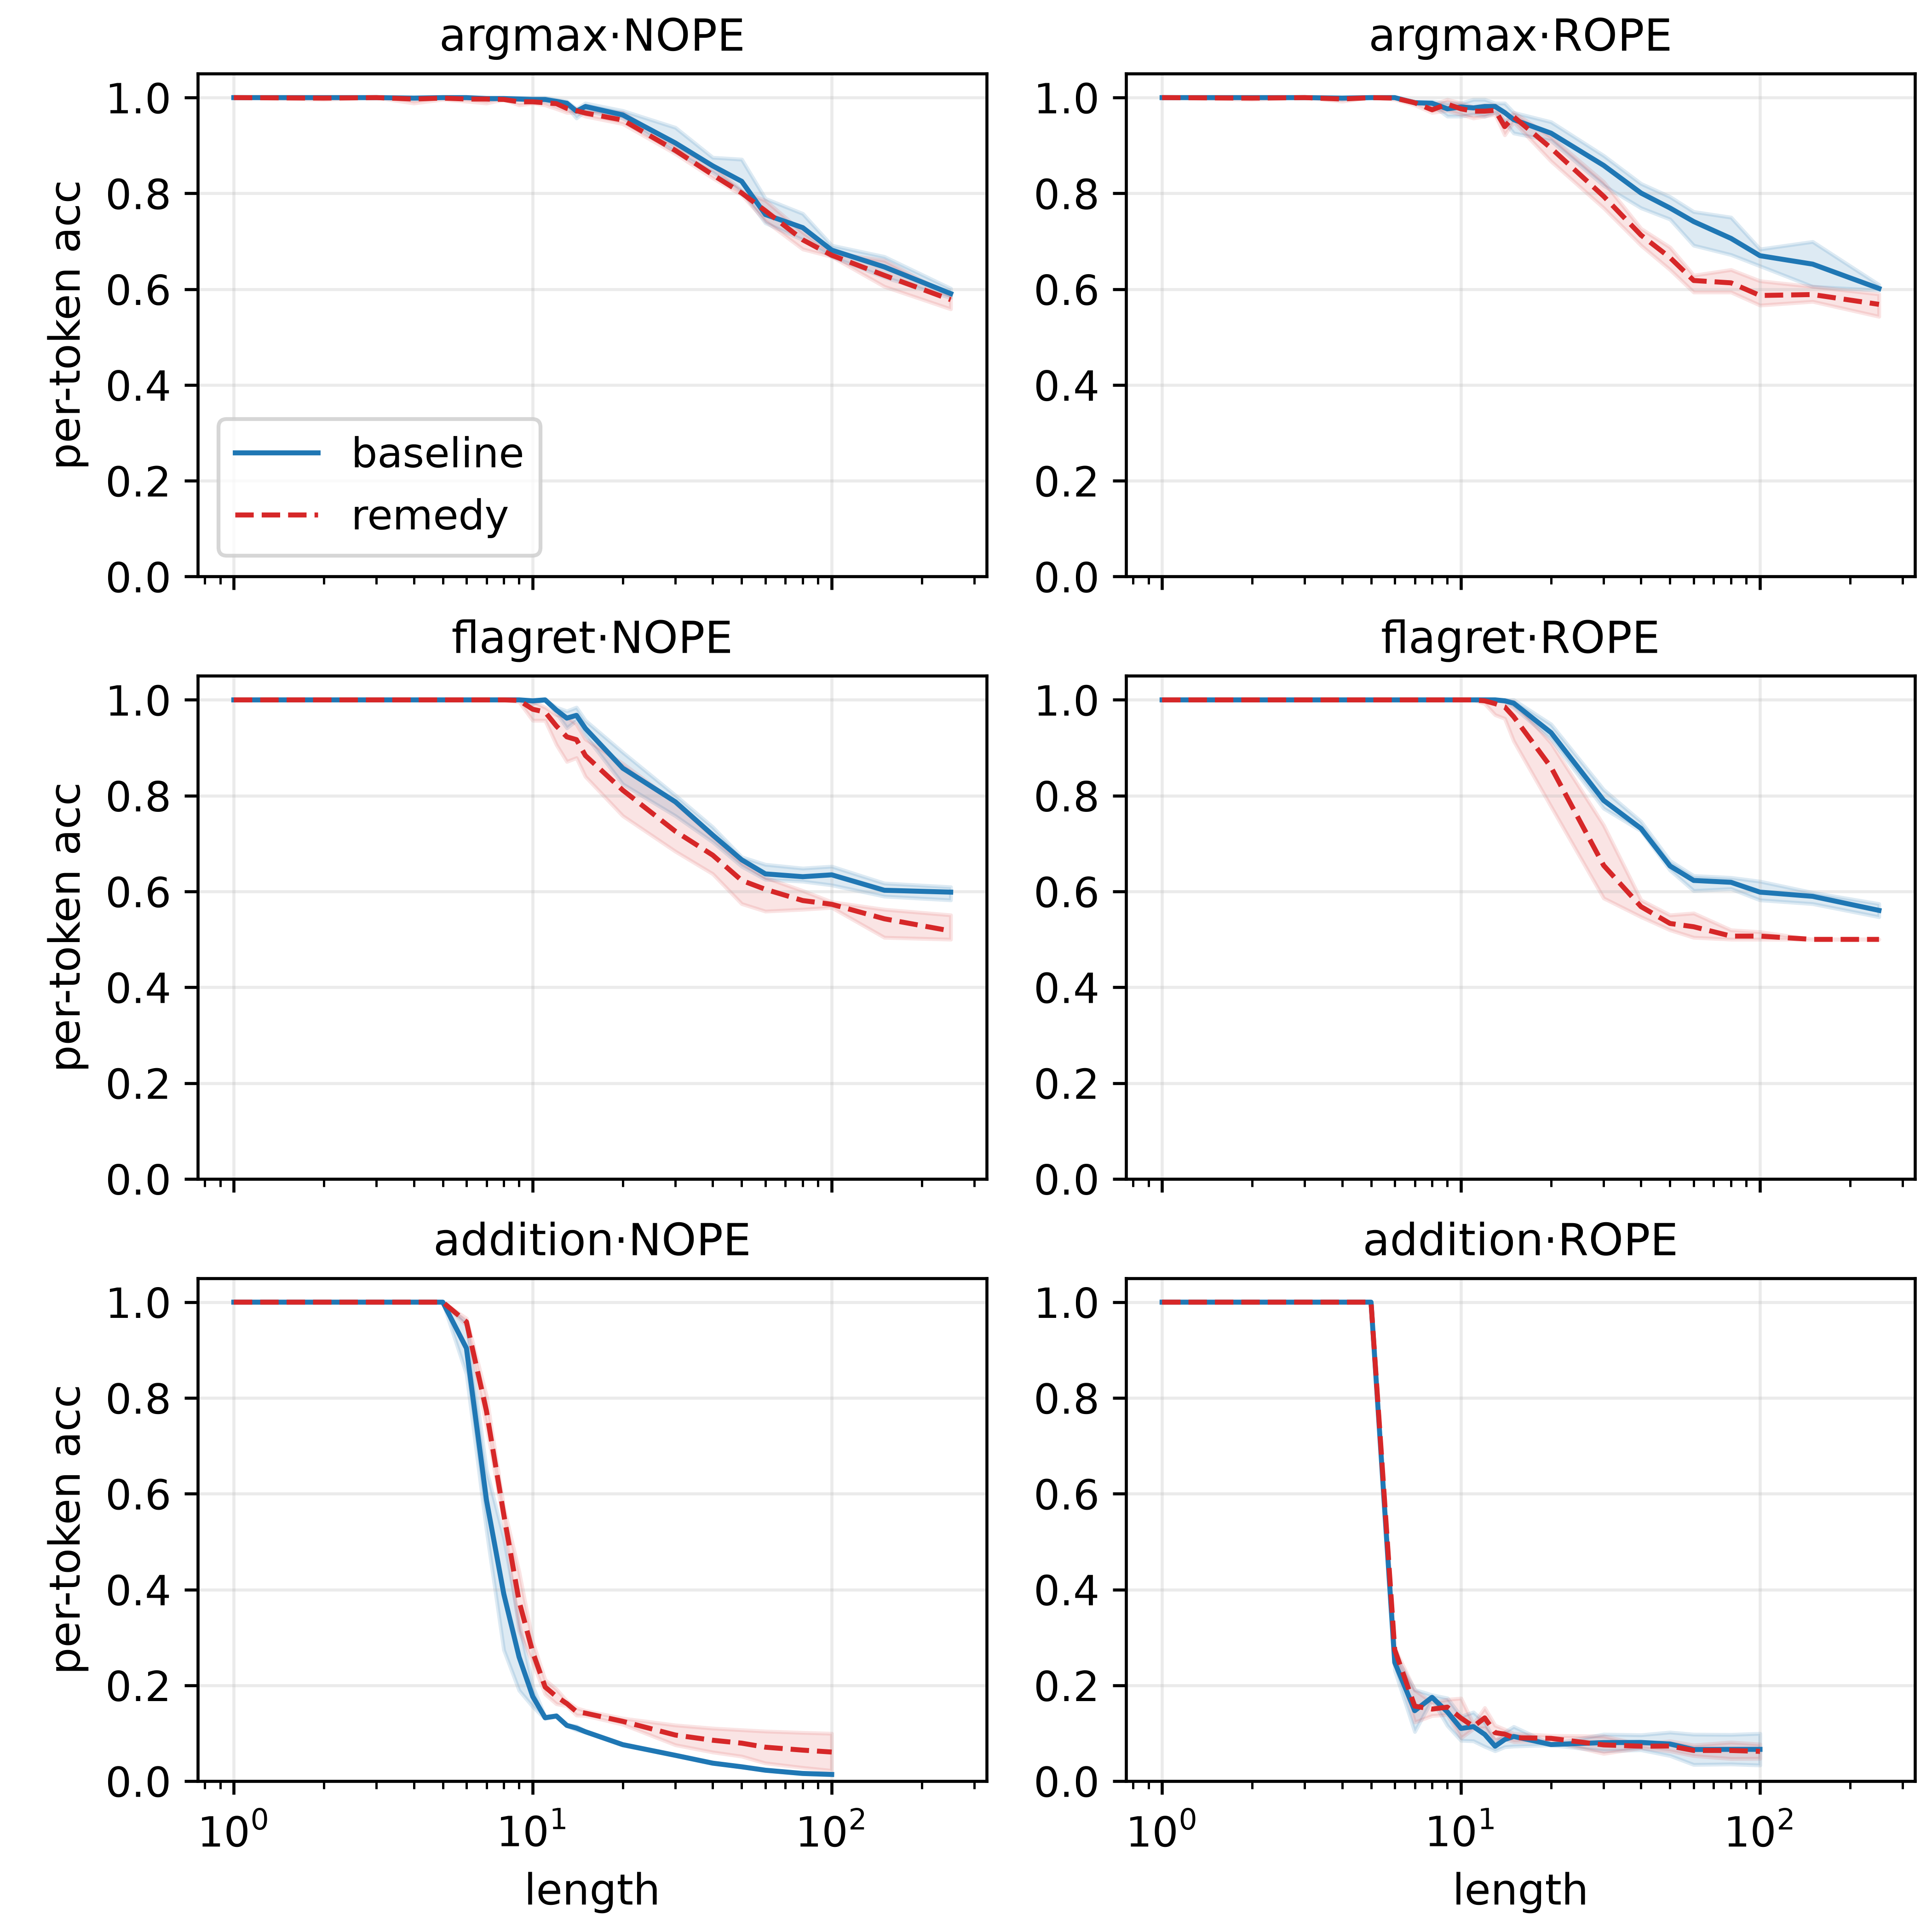
\includegraphics[width=0.82\textwidth]{figures/fig_accuracy_vs_length.png}
\caption{Accuracy across the full length ladder. The variance intervention lies at or below baseline in all
retrieval cells.}
\label{fig:supp-accuracy}
\end{figure*}

\subsection{Capacity, assignment, utility, and dose}

Across sixteen trained models, source-max raises accuracy by $0.153$ (95\% CI $[0.086,0.222]$), source-min
lowers it by $0.043$ ($[-0.058,-0.030]$), and the distractor control changes it by $0.011$
($[0.004,0.018]$). Source-max exceeds control in all 32 model--length comparisons. Maximum invariant error is
below $10^{-6}$. Increasing patched heads from one, two, four, to eight gives mean gains
$0.007$, $0.013$, $0.056$, and $0.153$, monotone in 31 of 32 comparisons.

At temperatures $\beta=1,2,4$, mean maximum weight rises from $0.362$ to $0.655$ and the source-max minus
source-min contrast rises from $0.196$ to $0.346$, an interaction of $+0.151$ ($[0.094,0.210]$).
Sharpening without reassignment changes accuracy by at most $+0.009$. Across $1{,}024$ examples, the local
utility term predicts finite margin changes with Pearson $0.917$, Spearman $0.989$, and $99.5\%$ sign
agreement. Active source utility gaps are positive in $89.2\%$ of head--example pairs.

Directly forcing source mass provides a separate dose response: at $50\times$ training length, baseline
accuracy is $0.59$ and rises monotonically toward one as forced source mass approaches one. This shows that
the routed source value is sufficient in the controlled task without implying that arbitrary source-max
swaps satisfy the utility condition.

\begin{figure}[t]
\centering
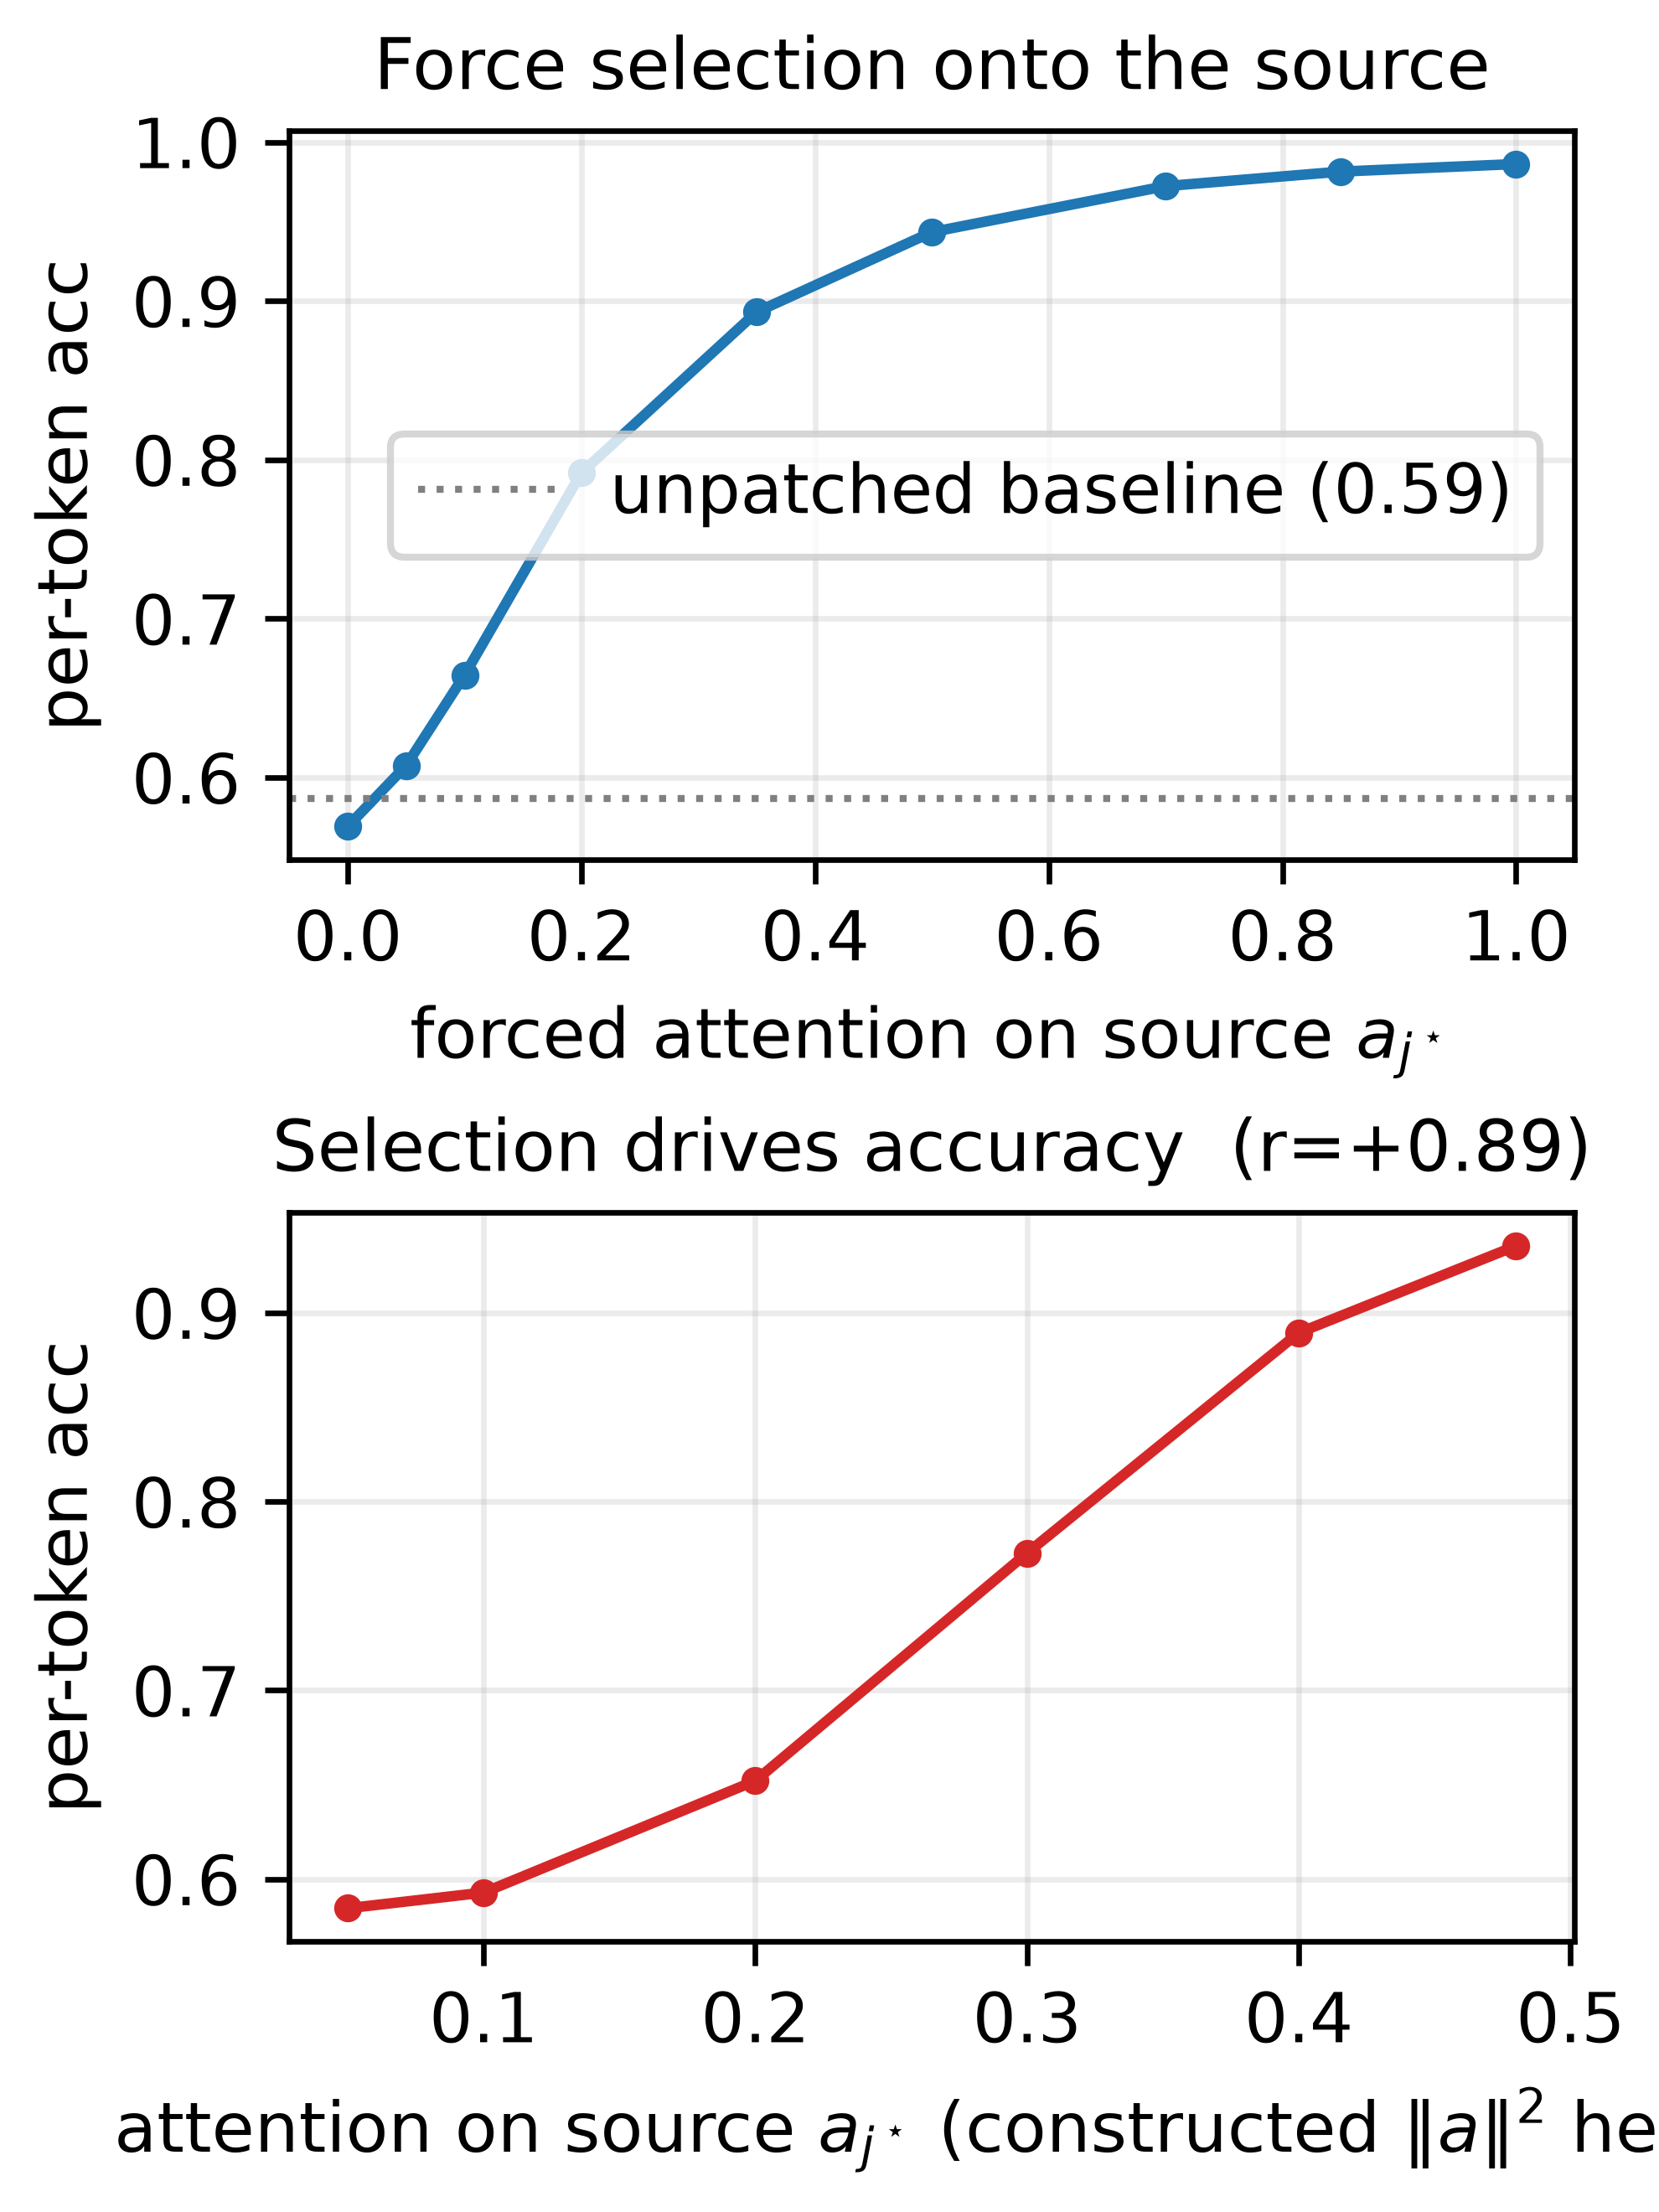
\includegraphics[width=0.96\columnwidth]{figures/fig_patch.png}
\caption{Direct manipulation of source attention. Accuracy rises monotonically with forced source mass.}
\label{fig:supp-patch}
\end{figure}

\subsection{Two-evidence computation and arity boundary}

Eight two-layer width-$128$ models reach perfect training competence on modular sum. At $5\times$ length,
evidence-max raises exact match by $0.066$, evidence-min lowers it by $0.291$, and the matched control changes
it by $0.023$. Evidence-max exceeds control by $0.043$ ($[0.017,0.072]$).

\begin{table}[t]
\centering
\small
\setlength{\tabcolsep}{3pt}
\begin{tabular}{lrrrrr}
\toprule
Length & Natural & Evid.-max & Evid.-min & Control & Max--ctrl. \\
\midrule
$2\times$ & .952 & .971 & .393 & .964 & +.007 \\
$5\times$ & .484 & .550 & .194 & .507 & +.043 \\
\bottomrule
\end{tabular}
\caption{Exact match on two-evidence modular sum, averaged over eight competent models.}
\label{tab:supp-multi}
\end{table}

The registered variable-evidence stage leaves arbitrary $r$ unestablished. Two- and three-evidence
models reach training competence, but the three-evidence max--control interval includes zero. Four-evidence
candidates fail the frozen competence gate: the largest eight-layer, width-$512$ candidate reaches
$0.748$ exact match against the required $0.8$. No four-evidence intervention is interpreted.

\section{Pretrained-Model Protocols and Results}

\subsection{Synthetic in-context recall}

Prompts contain key--value pairs followed by a query key. The source is the value paired with that key.
For each model, a calibration split selects a layer and $K$ heads; this circuit is frozen across disjoint
evaluation examples and lengths. We measure untouched accuracy, target-versus-competitor margin, and every
intervention invariant on paired examples. The family probe uses Pythia-1.4B, Qwen2.5-1.5B, and Gemma-2-2B;
causal tests additionally use Qwen2.5-7B NF4 and SmolLM2-1.7B.

\begin{figure*}[t]
\centering
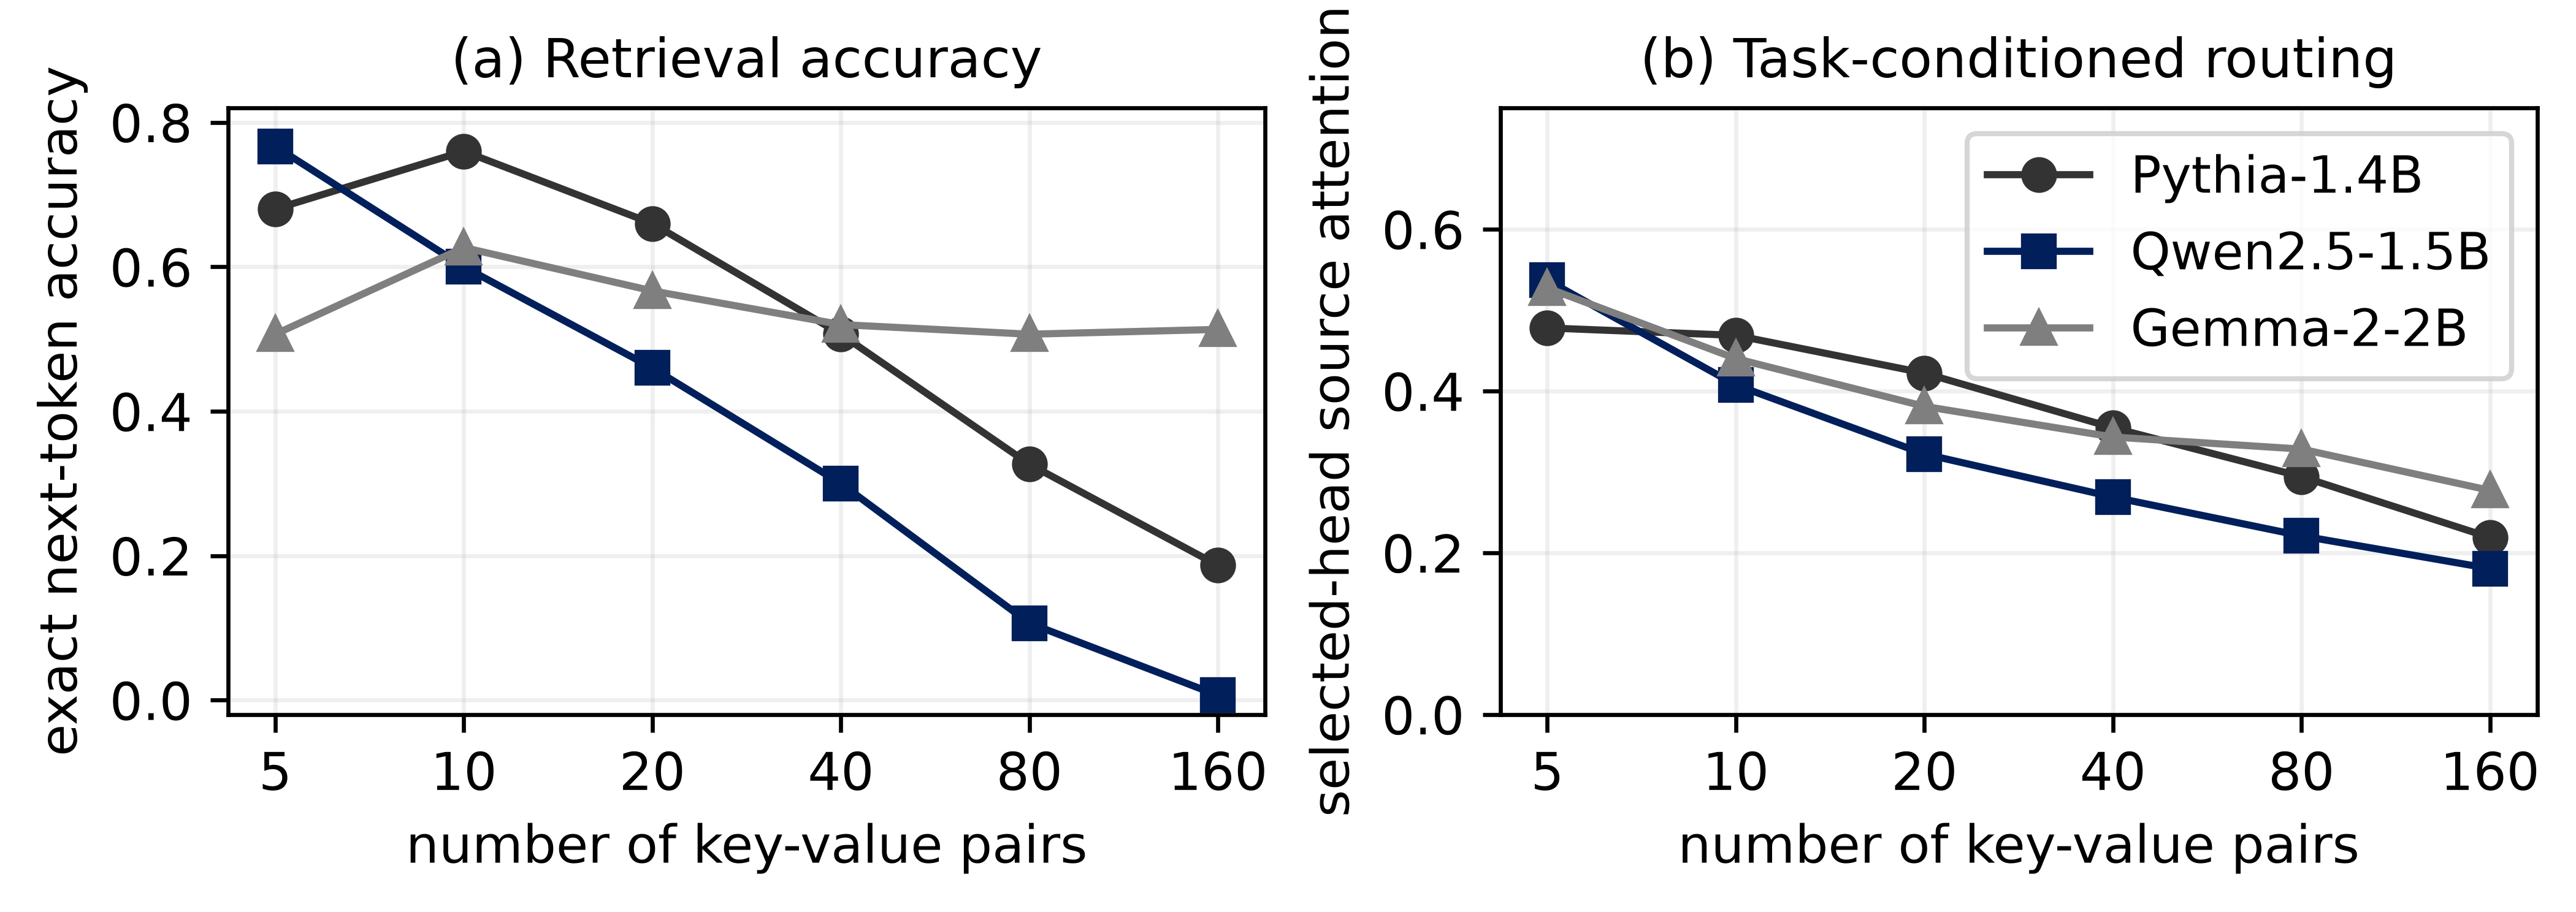
\includegraphics[width=0.92\textwidth]{figures/fig_realmodel_family.png}
\caption{Pretrained family sweep. Pythia and Qwen lose accuracy with length, while Gemma remains competent
despite declining selected-head source attention.}
\label{fig:supp-family}
\end{figure*}

\begin{table*}[t]
\centering
\small
\setlength{\tabcolsep}{2.5pt}
\begin{tabular}{lrrrrrrr}
\toprule
Model & $N$ & Base & \multicolumn{3}{c}{$\Delta$ accuracy} & \multicolumn{2}{c}{$\Delta$ margin} \\
\cmidrule(lr){4-6}\cmidrule(lr){7-8}
& & Acc. & Source-max & Source-min & Control & Source-max & Source-min \\
\midrule
Qwen-1.5B & 5   & .539 & +.102 & -.258 & -.016 & +1.177 & -1.406 \\
& 20  & .398 & +.188 & -.117 & +.023 & +2.268 & -1.191 \\
& 80  & .070 & +.109 & -.023 & +.000 & +2.527 & -.285 \\
& 160 & .008 & +.062 & +.000 & +.000 & +2.204 & -.148 \\
\midrule
Qwen-7B NF4 & 5  & .448 & +.021 & -.135 & +.010 & +.325 & -.988 \\
& 20 & .271 & +.135 & -.104 & +.010 & +.891 & -1.185 \\
& 80 & .010 & +.010 & -.010 & +.000 & +.654 & -.546 \\
\midrule
Pythia-1.4B & 5  & .359 & +.109 & -.250 & +.039 & +.878 & -2.480 \\
& 20 & .039 & +.039 & -.039 & -.016 & +1.195 & -.622 \\
& 80 & .000 & +.000 & +.000 & +.000 & +.405 & +.034 \\
\midrule
Gemma-2-2B & 5  & .758 & +.008 & -.094 & +.016 & +.041 & -1.680 \\
& 20 & .711 & +.016 & -.133 & -.008 & +.020 & -1.341 \\
& 80 & .742 & +.000 & -.117 & +.000 & +.058 & -1.096 \\
\midrule
SmolLM2-1.7B & 5  & .945 & +.008 & -.008 & -.008 & -.013 & -.133 \\
& 20 & .516 & -.016 & +.000 & +.008 & -.410 & -.190 \\
& 80 & .023 & +.000 & +.000 & +.000 & -.083 & -.012 \\
\bottomrule
\end{tabular}
\caption{Complete source-mass-selected intervention table. Qwen and Pythia show positive source-max
effects; Gemma is saturated; SmolLM2 is the preregistered negative replication.}
\label{tab:supp-pretrained}
\end{table*}

\subsection{Utility-conditioned circuit selection}

For every candidate head, the calibration split evaluates transferred source mass times the local
source--donor utility gap. Selecting the layer with the largest top-four sum rescues SmolLM2 over three seeds:
at five pairs, source-max minus control is $+0.702$ margin ($[0.529,0.858]$) and $+0.052$ accuracy, while the
source-mass selector changes margin by $-0.021$ ($[-0.057,0.014]$). The paired utility-minus-mass effect is
$+0.723$ ($[0.544,0.882]$).

The ten-seed equal-budget ablation compares source mass, transfer mass, utility gap, predicted utility gain,
source gradient, gradient magnitude, and deterministic random circuits. Source gradient ranks first at
$+0.750$ ($[0.682,0.819]$), utility gain second at $+0.600$ ($[0.482,0.712]$), utility gap third at
$+0.296$, and source mass is $-0.040$. Across Qwen, Pythia, and SmolLM2, no single selector wins every model;
output-conditioned selectors nevertheless beat task-agnostic source mass.

\begin{table*}[t]
\centering
\small
\setlength{\tabcolsep}{3.0pt}
\begin{tabular}{rrlrrl}
\toprule
Seed & $K$ & Circuit & Layer & Max--control $\Delta M$ & Paired 95\% interval \\
\midrule
0 & 2 & selected & 14 & +.641 & [.311,1.018] \\
0 & 4 & selected & 14 & +1.430 & [.919,2.003] \\
0 & 8 & selected & 14 & +1.418 & [.885,2.013] \\
0 & 4 & adjacent $-1$ & 13 & +.067 & [-.091,.231] \\
0 & 4 & adjacent $+1$ & 15 & -.355 & [-.568,-.181] \\
0 & 4 & random layer & 11 & -.093 & [-.227,.029] \\
\midrule
1 & 2 & selected & 14 & +.459 & [.167,.801] \\
1 & 4 & selected & 14 & +.981 & [.507,1.539] \\
1 & 8 & selected & 14 & +1.069 & [.584,1.598] \\
1 & 4 & adjacent $-1$ & 13 & +.049 & [-.085,.189] \\
1 & 4 & adjacent $+1$ & 15 & -.277 & [-.395,-.168] \\
1 & 4 & random layer & 21 & -.190 & [-.326,-.059] \\
\midrule
2 & 2 & selected & 14 & +.281 & [.025,.550] \\
2 & 4 & selected & 14 & +.749 & [.356,1.190] \\
2 & 8 & selected & 14 & +.835 & [.427,1.288] \\
2 & 4 & adjacent $-1$ & 13 & +.326 & [.146,.548] \\
2 & 4 & adjacent $+1$ & 15 & +.239 & [.065,.457] \\
2 & 4 & random layer & 7 & +.106 & [-.007,.223] \\
\bottomrule
\end{tabular}
\caption{Complete Qwen layer, head-budget, and calibration-seed robustness audit. All nine selected-circuit
intervals exclude zero; none of the three random-layer intervals does.}
\label{tab:supp-selection-robustness}
\end{table*}

\begin{table}[t]
\centering
\small
\setlength{\tabcolsep}{3.0pt}
\begin{tabular}{lrrr}
\toprule
Model & Positive cells & Mean Spearman & Sign agreement \\
\midrule
Qwen2.5-1.5B & 6/6 & .866 [.832,.898] & .805 \\
Pythia-1.4B & 6/6 & .544 [.500,.586] & .807 \\
Gemma-2-2B & 6/6 & .554 [.534,.582] & .714 \\
\bottomrule
\end{tabular}
\caption{Three-seed pretrained utility replication. Brackets give the range of seedwise source-max
Spearman correlations.}
\label{tab:supp-utility-replication}
\end{table}

\begin{table}[t]
\centering
\small
\setlength{\tabcolsep}{3.0pt}
\begin{tabular}{llrr}
\toprule
Model & Top selector & Effect & Utility rank \\
\midrule
Pythia-1.4B & utility gain & +.519 & 1 \\
SmolLM2-1.7B & utility gain & +1.253 & 1 \\
Qwen2.5-1.5B & utility gap & +1.493 & 2 \\
\bottomrule
\end{tabular}
\caption{Equal-budget cross-family selector audit. No selector wins all three families; output-conditioned
selectors lead each family.}
\label{tab:supp-selector-family}
\end{table}

Continuous interpolation supplies a dose control. At strengths $0,.25,.5,.75,1$, utility-selected source-max
minus matched distractor interpolation changes margin by $0.000$, $0.446$, $0.817$, $1.128$, and $1.417$.
Every one of five seedwise paths is nondecreasing.

\subsection{Natural multiple-choice QA}

The natural test uses four-choice questions with a gold passage and unrelated passages. An example is
eligible only if the model answers correctly with full context and the gold passage alone, but incorrectly
without context. This filtering defines a model-specific context-dependent subset and is not intended to
estimate average performance over the full dataset. Calibration and evaluation examples are disjoint. Across
the six selector-by-seed cells, the median absolute difference between mean treatment and matched-control
$L_1$ displacement was $2.24\times10^{-4}$, with a 95th percentile of $8.42\times10^{-4}$. On the locked
64-calibration/128-evaluation
design over three seeds, utility-selected source-max exceeds control by $+0.336$ margin
($[0.176,0.512]$). Source-mass selection is harmful at $-0.112$ ($[-0.188,-0.043]$). An eight-token greedy
audit changes neither first-answer accuracy nor repetition relative to control.

For the nested length ladder, the selected circuit is frozen at four passages before appending unrelated
passages. Table~\ref{tab:supp-ladder} reports hierarchical 32-minus-4 changes. Qwen loses performance while
source mass rises and rescue weakens. SmolLM2 loses performance while source mass falls and rescue remains
increase. This rejects source-mass loss or increasing rescue as a universal mechanism of natural-context
degradation.

\begin{table*}[t]
\centering
\small
\setlength{\tabcolsep}{3.0pt}
\begin{tabular}{lrrrr}
\toprule
Model & $\Delta$ baseline source mass & $\Delta$ margin & $\Delta$ accuracy & $\Delta$ rescue margin \\
\midrule
Qwen2.5-1.5B & +.000955 $[+.000141,+.002033]$ & -1.036 $[-1.397,-.698]$ & -.0469 $[-.0742,-.0234]$ & -.179 $[-.352,-.005]$ \\
SmolLM2-1.7B & -.0000736 $[-.0000989,-.0000519]$ & -.193 $[-.320,-.066]$ & -.1016 $[-.1563,-.0547]$ & +.018 $[-.027,+.066]$ \\
\bottomrule
\end{tabular}
\caption{Natural-QA 32-minus-4-passage changes with hierarchical 95\% intervals.}
\label{tab:supp-ladder}
\end{table*}

\subsection{Complete alternative-explanation audit}

\begin{table*}[!t]
\centering
\small
\setlength{\tabcolsep}{3.0pt}
\begin{tabular}{>{\raggedright\arraybackslash}p{0.16\textwidth}
                >{\raggedright\arraybackslash}p{0.23\textwidth}
                >{\raggedright\arraybackslash}p{0.38\textwidth}
                >{\raggedright\arraybackslash}p{0.14\textwidth}}
\toprule
Alternative & Experiment or matched control & Quantitative result & Conclusion \\
\midrule
Concentration changed & Exact invariant checks after every permutation & Sorted-spectrum error is \neutral{0} in controlled models and $\leq\neutral{4.77\times10^{-7}}$ in pretrained runs & \helpful{Excluded exactly} \\
Any perturbation helps & Distractor-only permutation on the same rows & Control $\Delta$accuracy is \neutral{+.011 [.004,.018]} versus source-max \helpful{+.153 [.086,.222]} & \helpful{Cannot explain main effect} \\
Total source mass suffices & Two-evidence mass-preserving reassignment & Evidence-max exceeds the same-mass control by \helpful{+.043 [.017,.072]} exact match & \helpful{Rejected} \\
Output variance is causal & Normalize post-attention variance while leaving routing untouched & Variance ratio returns to \neutral{.99--1.00}; $50\times$ $\Delta$accuracy remains \harmful{-.013 to -.081} & \helpful{Rejected} \\
Any layer works & Frozen selected, adjacent, and random-layer circuits & Selected Qwen cells average \helpful{+.874}; random layers average \neutral{-.059} & \helpful{Rejected} \\
Output-independent selection suffices & Equal-budget ten-seed selector ablation & Source gradient \utilityhelpful{+.750}, utility gain \utilityhelpful{+.600}, source mass \harmful{-.040} & \helpful{Rejected} \\
Calibration leakage drives the gain & Disjoint calibration/evaluation examples and seed-cluster intervals & Held-out natural QA gives \utilityhelpful{+.336 [.176,.512]} margin over control across three seeds & \helpful{Excluded by design} \\
One source-mass trajectory explains natural length failure & Frozen-circuit 4--32 passage ladder & Qwen $\Delta m_S$ \diagnostic{+.00095} while margin falls \harmful{-1.036}; SmolLM2 $\Delta m_S$ \diagnostic{-.00007} with flat rescue & \diagnostic{Universal account rejected; cause open} \\
The result extends to arbitrary evidence arity & Registered pair, triple, and quadruple study & Pair \helpful{+.043 [.017,.072]}; triple \neutral{-.001 [-.009,.008]}; quadruple misses competence & \diagnostic{Unresolved beyond two} \\
\bottomrule
\end{tabular}
\caption{The complete alternative-explanation audit links each claim to a matched experiment and result.}
\label{tab:supp-causal-audit}
\end{table*}

\section{Additional Boundaries}

The equals-sign second prompt format fails its competence gate in Qwen; the blinded arrow-format pilot also
fails full-run competence despite directional margin signs. These runs are excluded from causal
replications. Pythia and Qwen are floor-limited at their longest contexts, so margin is the interpretable
tail outcome. Qwen-7B is quantized. Gemma supplies a high-competence saturation boundary.

The natural-QA length result broadens the behavioral observation but narrows the mechanism. The conditional
fixed-spectrum theorem survives because it predicts effects only through transferred mass, value utility,
and curvature. What fails is the stronger proposition that natural length degradation must involve source-
mass loss or become increasingly rescuable by the same frozen circuit.

\section{Reproducibility}

\paragraph{Code and artifacts.}
The anonymous supplementary bundle contains the training and intervention code, all configurations and random
seeds, prompts, paired per-example outputs, competence-gate failures, invariant checks, preregistrations,
analysis scripts, and generated tables. The package regenerates every reported statistic and figure from the
included result artifacts without rerunning a model.

\paragraph{Data and models.}
The controlled tasks are generated from the included task generator and therefore require no external dataset.
Natural MCQA samples are constructed from the public SQuAD training split \citep{rajpurkar2016squad}; the
sampling seed and eligibility rule are included in the bundle. Pretrained probes use publicly released Qwen,
Pythia, Gemma, and SmolLM2 checkpoints, with exact identifiers, tokenizer settings, and precision recorded in
the result artifacts. Synthetic training uses one GPU. A public code and artifact archive will be released on
acceptance.

\bibliography{references}

\end{document}
